\documentclass{standalone}
\usepackage{tikz}
\usetikzlibrary{patterns, positioning}

\begin{document}
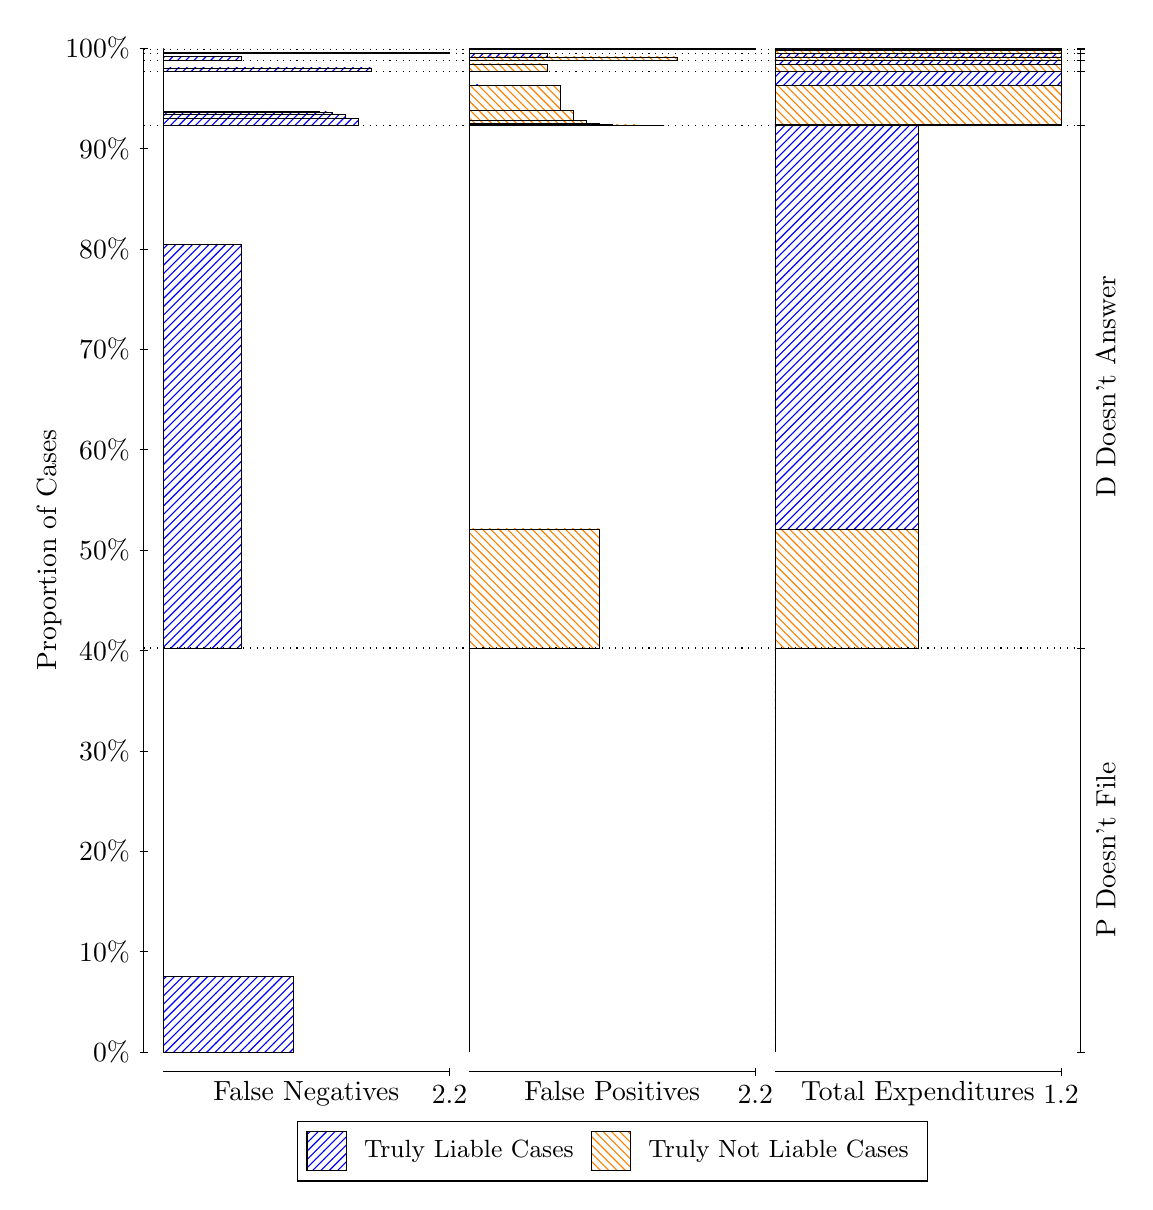
\begin{tikzpicture}
\draw[black, very thin] (1.5,1.75) -- (1.5,14.5);
\node[rotate=90, anchor=center] at (0.3, 8.125) {Proportion of Cases};
\draw[black, very thin] (1.45,1.75) -- (1.55,1.75);
\node[anchor=east] at (1.45, 1.75) {0\%};
\draw[black, very thin] (1.45,3.025) -- (1.55,3.025);
\node[anchor=east] at (1.45, 3.025) {10\%};
\draw[black, very thin] (1.45,4.3) -- (1.55,4.3);
\node[anchor=east] at (1.45, 4.3) {20\%};
\draw[black, very thin] (1.45,5.575) -- (1.55,5.575);
\node[anchor=east] at (1.45, 5.575) {30\%};
\draw[black, very thin] (1.45,6.85) -- (1.55,6.85);
\node[anchor=east] at (1.45, 6.85) {40\%};
\draw[black, very thin] (1.45,8.125) -- (1.55,8.125);
\node[anchor=east] at (1.45, 8.125) {50\%};
\draw[black, very thin] (1.45,9.4) -- (1.55,9.4);
\node[anchor=east] at (1.45, 9.4) {60\%};
\draw[black, very thin] (1.45,10.675) -- (1.55,10.675);
\node[anchor=east] at (1.45, 10.675) {70\%};
\draw[black, very thin] (1.45,11.95) -- (1.55,11.95);
\node[anchor=east] at (1.45, 11.95) {80\%};
\draw[black, very thin] (1.45,13.225) -- (1.55,13.225);
\node[anchor=east] at (1.45, 13.225) {90\%};
\draw[black, very thin] (1.45,14.5) -- (1.55,14.5);
\node[anchor=east] at (1.45, 14.5) {100\%};

\draw[black, very thin] (13.4,1.75) -- (13.4,14.5);
\draw[black, very thin] (13.35,1.75) -- (13.45,1.75);
\node[anchor=west] at (13.35, 1.75) {};
\draw[black, very thin] (13.35,6.8799) -- (13.45,6.8799);
\node[anchor=west] at (13.35, 6.8799) {};
\draw[black, very thin] (13.35,13.521) -- (13.45,13.521);
\node[anchor=west] at (13.35, 13.521) {};
\draw[black, very thin] (13.35,14.204) -- (13.45,14.204);
\node[anchor=west] at (13.35, 14.204) {};
\draw[black, very thin] (13.35,14.342) -- (13.45,14.342);
\node[anchor=west] at (13.35, 14.342) {};
\draw[black, very thin] (13.35,14.435) -- (13.45,14.435);
\node[anchor=west] at (13.35, 14.435) {};
\draw[black, very thin] (13.35,14.484) -- (13.45,14.484);
\node[anchor=west] at (13.35, 14.484) {};
\draw[black, very thin] (13.35,14.5) -- (13.45,14.5);
\node[anchor=west] at (13.35, 14.5) {};

\draw[black, very thin, pattern color=blue, pattern=north east lines] (1.75,1.75) rectangle (3.4015,2.7116);
\draw[black, very thin, pattern color=orange, pattern=north west lines] (1.75,2.7116) rectangle (1.75,6.8799);
\draw[black, very thin, pattern color=blue, pattern=north east lines] (1.75,6.8799) rectangle (2.7409,12.009);
\draw[black, very thin, pattern color=orange, pattern=north west lines] (1.75,12.009) rectangle (1.75,13.521);
\draw[black, very thin, pattern color=blue, pattern=north east lines] (1.75,13.521) rectangle (4.2273,13.603);
\draw[black, very thin, pattern color=blue, pattern=north east lines] (1.75,13.603) rectangle (4.0621,13.659);
\draw[black, very thin, pattern color=blue, pattern=north east lines] (1.75,13.659) rectangle (3.897,13.689);
\draw[black, very thin, pattern color=blue, pattern=north east lines] (1.75,13.689) rectangle (3.7318,13.692);
\draw[black, very thin, pattern color=blue, pattern=north east lines] (1.75,13.692) rectangle (3.5667,13.696);
\draw[black, very thin, pattern color=blue, pattern=north east lines] (1.75,13.696) rectangle (3.4015,13.697);
\draw[black, very thin, pattern color=blue, pattern=north east lines] (1.75,13.697) rectangle (3.2364,13.698);
\draw[black, very thin, pattern color=blue, pattern=north east lines] (1.75,13.698) rectangle (3.0712,13.698);
\draw[black, very thin, pattern color=blue, pattern=north east lines] (1.75,13.698) rectangle (2.9061,13.699);
\draw[black, very thin, pattern color=orange, pattern=north west lines] (1.75,13.699) rectangle (1.75,14.204);
\draw[black, very thin, pattern color=blue, pattern=north east lines] (1.75,14.204) rectangle (4.3924,14.247);
\draw[black, very thin, pattern color=orange, pattern=north west lines] (1.75,14.247) rectangle (1.75,14.342);
\draw[black, very thin, pattern color=blue, pattern=north east lines] (1.75,14.342) rectangle (2.7409,14.39);
\draw[black, very thin, pattern color=orange, pattern=north west lines] (1.75,14.39) rectangle (1.75,14.435);
\draw[black, very thin, pattern color=blue, pattern=north east lines] (1.75,14.435) rectangle (5.3833,14.443);
\draw[black, very thin, pattern color=orange, pattern=north west lines] (1.75,14.443) rectangle (1.75,14.484);
\draw[black, very thin, pattern color=orange, pattern=north west lines] (1.75,14.484) rectangle (1.75,14.492);
\draw[black, very thin, pattern color=blue, pattern=north east lines] (1.75,14.492) rectangle (1.75,14.5);
\draw[black, very thin, pattern color=orange, pattern=north west lines] (5.6333,1.75) rectangle (5.6333,5.9184);
\draw[black, very thin, pattern color=blue, pattern=north east lines] (5.6333,5.9184) rectangle (5.6333,6.8799);
\draw[black, very thin, pattern color=orange, pattern=north west lines] (5.6333,6.8799) rectangle (7.2848,8.3919);
\draw[black, very thin, pattern color=blue, pattern=north east lines] (5.6333,8.3919) rectangle (5.6333,13.521);
\draw[black, very thin, pattern color=orange, pattern=north west lines] (5.6333,13.521) rectangle (8.1106,13.521);
\draw[black, very thin, pattern color=orange, pattern=north west lines] (5.6333,13.521) rectangle (7.9455,13.522);
\draw[black, very thin, pattern color=orange, pattern=north west lines] (5.6333,13.522) rectangle (7.7803,13.523);
\draw[black, very thin, pattern color=orange, pattern=north west lines] (5.6333,13.523) rectangle (7.6152,13.525);
\draw[black, very thin, pattern color=orange, pattern=north west lines] (5.6333,13.525) rectangle (7.45,13.532);
\draw[black, very thin, pattern color=orange, pattern=north west lines] (5.6333,13.532) rectangle (7.2848,13.539);
\draw[black, very thin, pattern color=orange, pattern=north west lines] (5.6333,13.539) rectangle (7.1197,13.579);
\draw[black, very thin, pattern color=orange, pattern=north west lines] (5.6333,13.579) rectangle (6.9545,13.707);
\draw[black, very thin, pattern color=orange, pattern=north west lines] (5.6333,13.707) rectangle (6.7894,14.026);
\draw[black, very thin, pattern color=blue, pattern=north east lines] (5.6333,14.026) rectangle (6.4591,14.026);
\draw[black, very thin, pattern color=blue, pattern=north east lines] (5.6333,14.026) rectangle (6.2939,14.027);
\draw[black, very thin, pattern color=blue, pattern=north east lines] (5.6333,14.027) rectangle (6.1288,14.027);
\draw[black, very thin, pattern color=blue, pattern=north east lines] (5.6333,14.027) rectangle (5.9636,14.029);
\draw[black, very thin, pattern color=blue, pattern=north east lines] (5.6333,14.029) rectangle (5.7985,14.032);
\draw[black, very thin, pattern color=blue, pattern=north east lines] (5.6333,14.032) rectangle (5.6333,14.204);
\draw[black, very thin, pattern color=orange, pattern=north west lines] (5.6333,14.204) rectangle (6.6242,14.299);
\draw[black, very thin, pattern color=blue, pattern=north east lines] (5.6333,14.299) rectangle (5.6333,14.342);
\draw[black, very thin, pattern color=orange, pattern=north west lines] (5.6333,14.342) rectangle (8.2758,14.387);
\draw[black, very thin, pattern color=blue, pattern=north east lines] (5.6333,14.387) rectangle (6.6242,14.435);
\draw[black, very thin, pattern color=orange, pattern=north west lines] (5.6333,14.435) rectangle (5.6333,14.477);
\draw[black, very thin, pattern color=blue, pattern=north east lines] (5.6333,14.477) rectangle (5.6333,14.484);
\draw[black, very thin, pattern color=orange, pattern=north west lines] (5.6333,14.484) rectangle (9.2667,14.492);
\draw[black, very thin, pattern color=blue, pattern=north east lines] (5.6333,14.492) rectangle (7.6152,14.5);
\draw[black, very thin, pattern color=orange, pattern=north west lines] (9.5167,1.75) rectangle (9.5167,5.9184);
\draw[black, very thin, pattern color=blue, pattern=north east lines] (9.5167,5.9184) rectangle (9.5167,6.8799);
\draw[black, very thin, pattern color=orange, pattern=north west lines] (9.5167,6.8799) rectangle (11.333,8.3919);
\draw[black, very thin, pattern color=blue, pattern=north east lines] (9.5167,8.3919) rectangle (11.333,13.521);
\draw[black, very thin, pattern color=orange, pattern=north west lines] (9.5167,13.521) rectangle (13.15,13.528);
\draw[black, very thin, pattern color=blue, pattern=north east lines] (9.5167,13.528) rectangle (13.15,13.532);
\draw[black, very thin, pattern color=orange, pattern=north west lines] (9.5167,13.532) rectangle (13.15,14.028);
\draw[black, very thin, pattern color=blue, pattern=north east lines] (9.5167,14.028) rectangle (13.15,14.201);
\draw[black, very thin, pattern color=orange, pattern=north west lines] (9.5167,14.201) rectangle (13.15,14.203);
\draw[black, very thin, pattern color=blue, pattern=north east lines] (9.5167,14.203) rectangle (13.15,14.204);
\draw[black, very thin, pattern color=orange, pattern=north west lines] (9.5167,14.204) rectangle (13.15,14.299);
\draw[black, very thin, pattern color=blue, pattern=north east lines] (9.5167,14.299) rectangle (13.15,14.342);
\draw[black, very thin, pattern color=orange, pattern=north west lines] (9.5167,14.342) rectangle (13.15,14.387);
\draw[black, very thin, pattern color=blue, pattern=north east lines] (9.5167,14.387) rectangle (13.15,14.435);
\draw[black, very thin, pattern color=orange, pattern=north west lines] (9.5167,14.435) rectangle (13.15,14.477);
\draw[black, very thin, pattern color=blue, pattern=north east lines] (9.5167,14.477) rectangle (13.15,14.484);
\draw[black, very thin, pattern color=orange, pattern=north west lines] (9.5167,14.484) rectangle (13.15,14.492);
\draw[black, very thin, pattern color=blue, pattern=north east lines] (9.5167,14.492) rectangle (13.15,14.5);
\draw[black, dotted] (1.5,6.8799) -- (13.4,6.8799);
\draw[black, dotted] (1.5,13.521) -- (13.4,13.521);
\draw[black, dotted] (1.5,14.204) -- (13.4,14.204);
\draw[black, dotted] (1.5,14.342) -- (13.4,14.342);
\draw[black, dotted] (1.5,14.435) -- (13.4,14.435);
\draw[black, dotted] (1.5,14.484) -- (13.4,14.484);
\draw[black, very thin] (1.75,1.5) -- (5.3833,1.5);
\node[anchor=north] at (3.5667, 1.5) {False Negatives};
\draw[black, very thin] (5.3833,1.45) -- (5.3833,1.55);
\node[anchor=north] at (5.3833, 1.45) {2.2};

\draw[black, very thin] (5.6333,1.5) -- (9.2667,1.5);
\node[anchor=north] at (7.45, 1.5) {False Positives};
\draw[black, very thin] (9.2667,1.45) -- (9.2667,1.55);
\node[anchor=north] at (9.2667, 1.45) {2.2};

\draw[black, very thin] (9.5167,1.5) -- (13.15,1.5);
\node[anchor=north] at (11.333, 1.5) {Total Expenditures};
\draw[black, very thin] (13.15,1.45) -- (13.15,1.55);
\node[anchor=north] at (13.15, 1.45) {1.2};

\node[black, centered, rotate=90] at (13.72, 4.315) {P Doesn't File};
\node[black, centered, rotate=90] at (13.72, 10.2) {D Doesn't Answer};






\draw (7.449999999999999,1.5) node[draw=none] (baseCoordinate) {};
\begin{scope}[align=center]
        \matrix[scale=0.5, draw=black, below=0.5cm of baseCoordinate, nodes={draw}, column sep=0.1cm]{
            \node[rectangle, draw, minimum width=0.5cm, minimum height=0.5cm, pattern=north east lines, pattern color=blue] {}; &
            \node[draw=none, font=\small] (B) {Truly Liable Cases}; &
            \node[rectangle, draw, minimum width=0.5cm, minimum height=0.5cm, pattern=north west lines, pattern color=orange] {}; &
            \node[draw=none, font=\small] (B) {Truly Not Liable Cases}; \\
            };
\end{scope}

\end{tikzpicture}
\end{document}